\section{Description of Datasets}
\label{sec:methods/section_a}

To our understanding, there is no public or open source dataset of uncompressed video sequences with ground truths. Our group members prepared the uncompressed video sequences and annotated them to obtain ground truths in YOLO format. The existing ground truths prepared by the our group members are suitable for the object detection; however, for the purpose of analyzing the tracking performance, we further annotate the unique object identifiers (IDs) on the existing ground truths using Normalized Cross-correlation (NCC).
\begin{table}[htb]
    \centering
    \caption{List of Video Sequences \cite{choi_vcm_2020}}
    \begin{tabular}{|| c | c | c | c | c | c ||}
         \hline
          Sequence Class & Sequence Name & Frame Count & Resolution & Frame rate (Hz) & Bit depth  \\ [0.5ex]
         \hline\hline
          B & BasketballDrive & 500 & 1920x1080 & 50 & 8 \\ 
         \hline
          B & Cactus & 500 & 1920x1080 & 50 & 8 \\ 
         \hline
          B & Kimono & 240 & 1920x1080 & 24 & 8 \\
         \hline
          B & ParkScene & 240 & 1920x1080 & 24 & 8 \\
         \hline
          C & BasketballDrill & 500 & 832x480 & 50 & 8 \\
         \hline
          C & PartyScene & 500 & 832x480 & 50 & 8 \\
         \hline
          C & RaceHorses & 300 & 832x480 & 30 & 8 \\
         \hline
          D & BasketballPass & 500 & 416x240 & 50 & 8 \\
         \hline
          D & BlowingBubbles & 500 & 416x240 & 50 & 8 \\
          \hline
          D & RaceHorses & 500 & 416x240 & 30 & 8 \\
          \hline
          E & KristenAndSara & 600 & 1280x720 & 60 & 8 \\
          \hline
          E & Johnny & 600 & 1280x720 & 60 & 8 \\
          \hline
          E & FourPeople & 600 & 1280x720 & 60 & 8 \\
          \hline
    \end{tabular}
    \label{tab:seq_list}
\end{table}
Table \ref{tab:seq_list} shows the 13 uncompressed video sequences with prepared ground truths out of 17 available video sequences from \cite{choi_vcm_2020}. The object tracking pipeline consists of YOLOv3 detector and SORT as shown in Figure \ref{fig:yolov3+SORT}. 
\begin{figure}[!htbp]
  \centering
  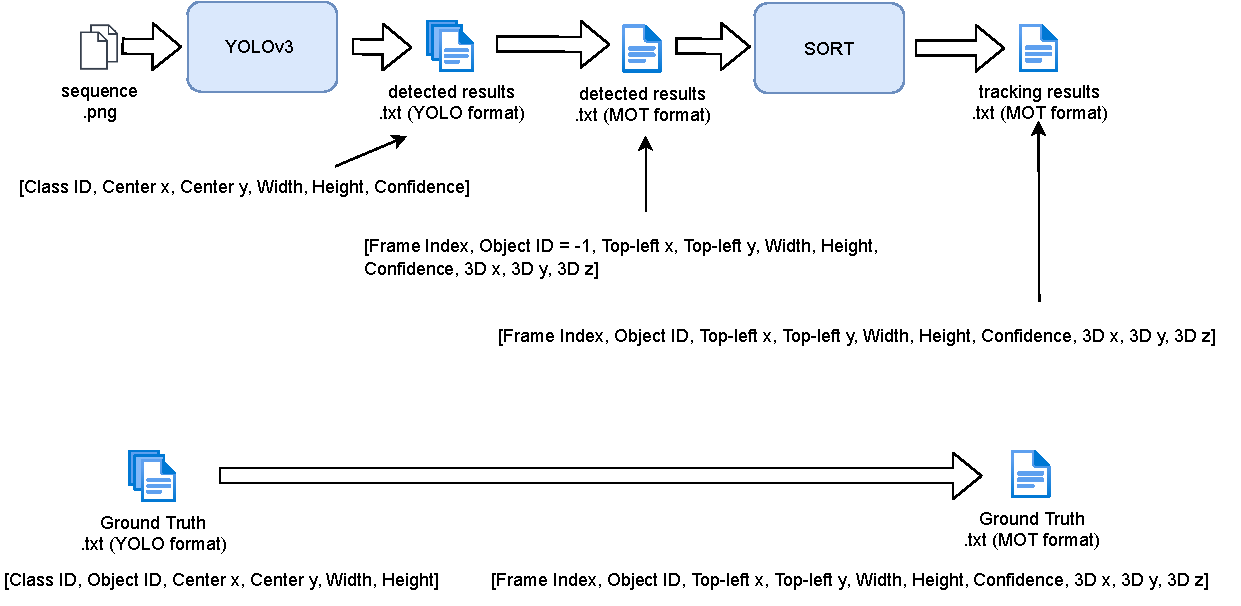
\includegraphics[width=1.0\linewidth]{img/YOLOv3+SORT.pdf}
  \caption[Object tracking pipeline with YOLO v3 and SORT]
  {Object tracking pipeline with YOLO v3 and SORT.}
  \label{fig:yolov3+SORT}
\end{figure}
Input video sequence of png files are input to the YOLOv3 object detector. The output from YOLOv3 as detected results will be generated in YOLO format as [Class ID, Center x, Center y, Width, Height, Confidence]. Class ID indicates the identifier to the type of class; for example, person as 0, sports ball as 32, and chair as 56, which are part of the 80 COCO classes. Center x and Center y are center position of bounding box, width and height are the corresponding dimension of boxes. Confidence indicates the score of how confident the object is detected. These results are converted to MOT format accepted in 2015 MOT benchmark from \textit{MOTChallenge}. The object IDs, the unique identifiers to the objects, for the detected results are initialized as -1. Applying SORT to this detected result, we obtain the tracking result in MOT format with the assigned object IDs as [Frame index, Object ID, Top-left x, Top-left y, Width, Height, Confidence, 3D x, 3D y, 3D z]. Top-left x and Top-left y is the position of bounding box at the top-left corner. 3D x, 3D y, 3D z is the position of the bounding box in 3D dimension but we assigned -1 in our experiment since the real-world position is not applicable to our experiment. The ground truths are also converted from YOLO format to MOT format.

% The MOT format from \textit{MOTChallenge} is summarized in 
% \begin{myfont}
% \centering
% Class ID, Object ID, center X, center Y, Width, Height
% \end{myfont}


% \begin{table}[]
%     \centering
%     \caption{}
%     \begin{tabular}{|c|c|}
%         \hline
%         Data field & Description \\
%         \hline\hline
%         Frame Index & Frame index in a sequence \\
%         \hline
%         Object ID & Unique identifier to the object \\
%         \hline
%         Top-left x & x coordinate in top-left corner of the bounding box \\
%         \hline
%         Top-left y & y coordinate in top-left corner of the bounding box \\
%         \hline
%         Width & Width of the bounding box \\
%         \hline
%         Height & Height of the bounding box \\
%         \hline
%         Confidence & Confidence score of the detection of the object \\
%         \hline
%         3D x & x coordinate in 3D bounding box \\
%         \hline
%         3D y & y coordinate in 3D bounding box \\
%         \hline
%         3D z & z coordinate in 3D bounding box \\
%         \hline
%     \end{tabular}
%     \label{tab:MOT_format}
% \end{table}


